\begin{name}
	{\tenchude}
	{\tendethi}
	{\tentruong}
	{\thoigian}
\end{name}
\setcounter{ex}{0}\setcounter{bt}{0}
\TN
\Opensolutionfile{ans}[ans/ansDe3-TN3]
\begin{ex}%[2-D1B1-SO-3-2425]%[VN-MT-7, Nguyễn Khánh Trọng]%[2D1N1-1]
	Hàm số $y=-x^3+3x$ đồng biến trên khoảng nào dưới đây?
	\choice
	{\True $(-1;1)$}
	{$(-\infty;-1)$}
	{$\left(0;\sqrt{3}\right)$}
	{$(1;+\infty)$}
	\loigiai{
		Tập xác định $\mathscr{D}=\mathbb{R}$.\\
		Ta có $y=-x^3+3x\Rightarrow y'=-3x^2+3$.\\
		$y'=0\Leftrightarrow x=\pm 1$.\\
		Bảng biến thiên
		\begin{center}
			
\begin{tikzpicture}
				\tkzTabInit[nocadre=true, lgt=1.0, espcl=3, deltacl=0.5]
				{$x$ /.7, $y'$ /.7, $y$ /2}
				{$-\infty$,$-1$,$1$,$+\infty$}
				\tkzTabLine{ ,-,z,+,z,-, }
				\tkzTabVar{+/$+\infty$,-/$-2$,+/$2$,-/$-\infty$}
			\end{tikzpicture}
		\end{center}
		Từ bảng biến thiên ta thấy hàm số đồng biến trên khoảng $(-1;1)$.}
\end{ex}

\begin{ex}%[Dự án 2025 - đề cấu trúc mới, Hung Doan]%[2D1N1-2]
	\immini{Hàm số $y=f(x)$ có đồ thị như hình vẽ. Hàm số $y=f(x)$ đồng biến trên khoảng nào dưới đây?
		\choice
		{$(-1;1)$}
		{$(0;2)$}
		{\True $(-2;-1)$}
		{$(-2;1)$}}{
		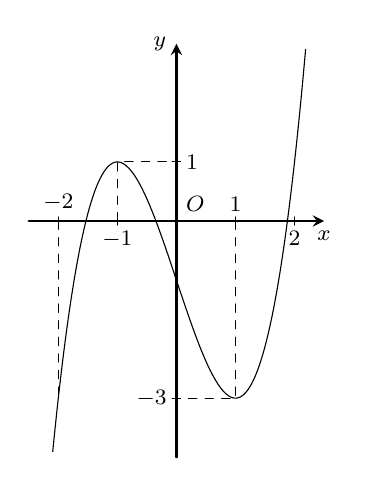
\begin{tikzpicture}[scale=0.75, font=\footnotesize, line join=round, line cap=round, >=stealth]
			\def\xt{-2.5} \def\xp{2.5} \def\yt{3} \def\yd{-4}
			\draw[->,  line width=0.8pt](\xt, 0)--(\xp, 0) node[below]{$x$};
			\draw[->,  line width=0.8pt](0,\yd)--(0,\yt) node[left]{$y$};
			\node at (0, 0) [above right]{$O$};
			\clip(\xt+0.1,\yd+0.1) rectangle(\xp-0.1,\yt-0.1);
			\draw[ smooth,samples=300] plot(\x,{(\x)^3-3*(\x)-1});
			\foreach \x in {-2,1}
			\draw[shift ={ (\x,0)}]node[above]{$\x$} (0pt,2pt) --(0pt,-2pt);
			\foreach \x in {-1,2}
			\draw[shift ={ (\x,0)}]node[below]{$\x$} (0pt,2pt) --(0pt,-2pt);
			\draw[shift ={ (0,-3)}]node[left]{$-3$} (2pt,0pt) --(-2pt,0pt);
			\draw[shift ={ (0,1)}]node[right]{$1$} (2pt,0pt) --(-2pt,0pt);
			\draw[dashed] (-2,0) -- (-2,-3);
			\draw[dashed] (-1,0) -- (-1,1) -- (0,1);
			\draw[dashed] (1,0) -- (1,-3) -- (0,-3);
		\end{tikzpicture}
	}
	\loigiai{
		Từ đồ thị ta thấy trên khoảng $(-2;-1)$ đồ thị đi lên do đó hàm số đồng biến trên khoảng $(-2;-1)$.}
\end{ex}

\begin{ex}%[2D1V1-5]%[Tổ 16 - Đợt 16 - Chương 1 - - KNTT - Đề 3]%[Nguyễn Kiều Nhã Tú]
	Một chất điểm chuyển động theo quy luật $S=-\dfrac{1}{3}t^3+4t^2+9t$ với $t \geq 0$ (giây) là khoảng thời gian tính từ lúc vật bắt đầu chuyển động và $S$ (mét) là quãng đường vật chuyển động trong thời
	gian đó. Hỏi trong khoảng thời gian 10 giây, kể từ lúc bắt đầu chuyển động, khoảng thời gian nào vận tốc của vật tăng?
	\choice
	{$(0;5)$}
	{\True $(0;4)$}
	{$(4;10)$}
	{$(3;10)$}
	\loigiai
	{
	Ta có vận tốc của vật $v(t)=S'(t)=-t^2+8 t+9$, $t \in(0;10)$.\\
	$v'(t)=-2t+8$. Xét $v'(t)=0 \Rightarrow t=4 \in (0;10)$.\\
	Bảng biến thiên
	\begin{center}
		\begin{tikzpicture}[font=\normalsize,t style/.style={style=solid}]
			%dòng khai báo
			\tkzTabInit[nocadre=true,lgt=1.2,espcl=2.5,deltacl=0.5]
			{$t$/0.75,$v'(t)$/0.75, $v(t)$/2}
			{$0$, $4$, $10$}
			%dòng xét dấu của đạo hàm
			\tkzTabLine{,+, 0,-,} % z, t, d, h (h: tô miền);
			%Khai báo vị trị các điểm của dòng f(x)
			\path ($(N12)!0.9!(N13)$) node (A1){$ v(0) $}
			($(N22)!0.2!(N23)$) node (A2){$ 25 $}
			($(N32)!0.9!(N33)$) node (A3){$ v(10) $};
			\foreach \x/\y in {A1/A2,A2/A3}{
					\draw[-stealth] (\x)--(\y);
				}
		\end{tikzpicture}
	\end{center}
	Từ bảng biến thiên ta có trong khoảng thời gian $(0;4)$ thì vận tốc của vật tăng.
	}
\end{ex}

\begin{ex}%[Lê Hữu Kiệt]%[2D1N2-1]
	Cho hàm số $y=\dfrac{x^3}{3}-2x^2+3x+\dfrac{2}{3}$. Điểm cực đại của đồ thị hàm số là:
	\choice
	{$x=1$}
	{$\left(3;\dfrac{2}{3} \right)$}
	{$x=3$}
	{\True $(1;2)$}
	\loigiai{
		Tập xác định $\mathscr{D}=\mathbb{R}$.\\
		Ta có $y'=x^2-4x+3$. Khi đó $y'=0 \Leftrightarrow x^2-4x+3=0 \Leftrightarrow \hoac{& x= 1 \\ & x=3.}$\\
		Bảng biến thiên
		\begin{center}
			
\begin{tikzpicture}[>=stealth]
				\tkzTabInit[espcl=2]
				{$x$/0.7, $y'$/0.7, $y$/2}
				{$-\infty$, $1$, $3$, $+\infty$}
				\tkzTabLine
				{, + , $0$ , - , $0$ , + , }
				\tkzTabVar
				{-/$-\infty$, +/$2$, -/$\dfrac{2}{3}$, +/$+\infty$}
			\end{tikzpicture}
		\end{center}
		Từ bảng biến thiên, điểm cực đại của đồ thị hàm số là $(1;2)$.
	}
\end{ex}

\begin{ex}%[2D1N2-2]%[CTST - Lớp 12 - Ôn tập cuối học kì 1 - Đề 5]%[Don Lee]
	\immini
	{Cho hàm số $f(x)=ax^3+bx^2+cx+d$ có đồ thị là đường cong như hình vẽ. Hàm số đạt cực tiểu tại
		\choice
		{$y=0$}
		{\True $x=2$}
		{$x=0$}
		{$y=-2$}}
	{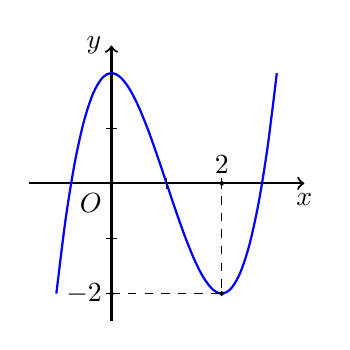
\begin{tikzpicture}[scale=0.7]
			\draw[->, thick] (-1.5,0)--(3.5,0) node[below] {$x$};
			\draw[->, thick] (0,-2.5)--(0,2.5) node[left] {$y$};
			\draw[domain=-1:3,smooth,variable=\x,blue,thick] plot ({\x},{(\x)^3-3*(\x)^2+2});
			\draw[dashed] (0,-2)-|(2,0);
			\foreach \x in {0,1,2}
			\draw (\x,-0.1)--(\x,0.1);
			\foreach \y in {-2,-1,1,2}
			\draw (-0.1,\y)--(0.1,\y);
			\filldraw (0,0) circle (1pt) node[below left] {$O$};
			\filldraw (0,-2) circle (1pt) node[left] {$-2$};
			\filldraw (2,0) circle (1pt) node[above] {$2$};
			\filldraw (2,-2) circle (1pt);
		\end{tikzpicture}}
	\loigiai{
		Hàm số đạt cực tiểu tại $x=2$.
	}
\end{ex}

\begin{ex}%[Trần Xuân Hòa]%[2D1H2-1]
	Cho hàm số $y=\dfrac{x^2+3}{x-1}$. Khẳng định nào sau đây là đúng?
	\choice
	{Hàm số đạt cực tiểu tại $x=-1$}
	{\True Hàm số có hai cực trị thỏa $y_\text{{CĐ}}<y_{C T}$}
	{Hàm số đạt cực đại tại $x=3$}
	{Giá trị cực tiểu bằng $-2$}
	\loigiai{Tập xác định $\mathscr{D}=\mathbb{R}\setminus \{1\}$.\\
		Ta có $y=x+1+\dfrac{4}{x-1}$ nên $y'=\dfrac{x^2-2x-3}{(x-1)^2}$ và $y'=0\Rightarrow \hoac{&x=-1\\&x=3}$. Bảng biến thiên
		\begin{center}
			
\begin{tikzpicture}
				\tkzTabInit[espcl=3,lgt=1.5]
				{$x$/0.7,$y'$/0.7,$y$/2.1}
				{$-\infty$,$-1$,$1$,$3$,$+\infty$}
				\tkzTabLine{,+,0,-,d,-,0,+,}
				\tkzTabVar{-/$-\infty$,+/$-2$,-D+/$-\infty$/$+\infty$,-/$6$,+/$+\infty$}
			\end{tikzpicture}
		\end{center}
		Từ bảng biến thiên, ta có $y_\text{CĐ}=-2$, $y_\text{CT}=6$. Do vậy $y_\text{CĐ}<y_\text{CT}$.
	}
\end{ex}

\begin{ex}%[2D1H3-1]
	Với giá trị nào của $m$ thì hàm số $y=\dfrac{mx-1}{x+m}$ đạt giá trị lớn nhất bằng $\dfrac{1}{3}$ trên $\left[ 0;2 \right]$.
	\choice
	{ $m=-1$}
	{\True $m=1$}
	{ $m=-3$}
	{ $m=3$}
	\loigiai{
		Ta có tập xác định $\mathscr{D}=\mathbb{R}\setminus \{-m\}$.\\
		$y^\prime=\dfrac{m^2+1}{\left(x+m\right)^2}>0 ~ \forall x\neq -m$.\\
		Hàm số luôn đồng biến trên từng khoảng xác định.\\
		Hàm số đạt giá trị lớn nhất bằng $\dfrac{1}{3}$ trên $\left[ 0;2 \right]$ khi $\heva{&y\left(2\right)=\dfrac{1}{3}\\&\hoac{&-m<0\\&-m>2}}\Leftrightarrow \heva{&\dfrac{2m-1}{2+m}=\dfrac{1}{3}\\&\hoac{&-m<0\\&-m>2}}\Leftrightarrow m=1$.
	}
\end{ex}

\begin{ex}%[2D1N4-1]
	Cho các hằng số $a$, $b$, $c$, $d$ khác $0$ thoả mãn $a d-b c \neq 0$. Đồ thị của hàm số $y=\dfrac{a x+b}{c x+d}$ có đường tiệm cận đứng và tiệm cận ngang là
	\choice
	{$x=\dfrac{d}{c}, y=\dfrac{a}{c}$}
	{\True $x=\dfrac{-d}{c}, y=\dfrac{a}{c}$}
	{$x=\dfrac{-d}{c}, y=\dfrac{b}{d}$}
	{$x=\dfrac{-b}{a}, y=\dfrac{b}{d}$}
	\loigiai{
		Ta có $\lim \limits_{x\to \pm \infty}y=\dfrac{a}{c}$. Nên đồ thị của hàm số $y=\dfrac{a x+b}{c x+d}$  có tiệm cận ngang là $y=\dfrac{a}{c}$.\\
		Và $\lim \limits_{x\to \pm -\tfrac{d}{c}}y=\infty$. Nên đồ thị của hàm số $y=\dfrac{a x+b}{c x+d}$ có đường tiệm cận đứng là $x=\dfrac{-d}{c}$. }
\end{ex}

\begin{ex}%[Dự án TL12New-4in1-NCT]%[2D1H4-1]
	Cho hàm số $ y=f(x) $ có bảng biến thiên như sau:
	\begin{center}
		
\begin{tikzpicture}
			\tkzTabInit[nocadre=false,lgt=1.2,espcl=2,deltacl=0.6]
			{$x$ /0.6,$y’$ /0.6,$y$ /2}
			{$-\infty$,$-2$,$+\infty$}
			\tkzTabLine{,-,d,-,}
			\tkzTabVar{+/$-1$,-D+/$-\infty$/$+\infty$,-/$-1$}
		\end{tikzpicture}
	\end{center}
	Tiệm cận ngang của đồ thị hàm số đã cho là đường thẳng  có phương trình
	\choice
	{\True $ y=-1 $}
	{$ y=-2 $}
	{$ x=-2 $}
	{$ x=-1 $}
	\loigiai
	{
		Ta thấy $ \lim \limits_{x \to \pm \infty} f(x) =-1$ nên đồ thị hàm số có tiệm cận ngang là đường thẳng $ y=-1 $.
	}
\end{ex}

\begin{ex}%[BG-12NEW-4in1, Nguyen Huynh]%[2D1V4-1]
	Tiệm cận ngang của đồ thị hàm số $y = \sqrt{4x^2-8x+5} + 2x$ có phương trình là
	\choice
	{$y=4$}
	{$y=-2$}
	{\True $y=2$}
	{$y=-4$}
	\loigiai
	{
		Hàm số đã cho xác định khi và chỉ khi $4x^2-8x+5\ge0$ (đúng với mọi $x\in\mathbb{R}$).\\
		Ta có
		\begin{itemize}
			\item $\lim\limits_{x\to+\infty}y=+\infty$.
			\item $\lim\limits_{x\to-\infty}y=\lim\limits_{x\to-\infty}\dfrac{-8x+5}{\sqrt{4x^2-8x+5}-2x}=\lim\limits_{x\to-\infty}\dfrac{-8+\dfrac{5}{x}}{-\sqrt{4-\dfrac{8}{x}+\dfrac{5}{x^2}}-2}=2$.
		\end{itemize}
		Vậy đồ thị hàm số đã cho có đường tiệm cận ngang là $y=2$.
	}
\end{ex}

\begin{ex}%[2D1N5-1]%[CTST - Lớp 12 - Ôn tập cuối học kì 1 - Đề 5]%[Don Lee]
	\immini
	{Đồ thị của hàm số nào dưới đây có dạng như đường cong trong hình vẽ?
		\choice
		{$y=x^4-3x^2+1$}
		{$y=x^4-2x^2+1$}
		{\True $y=-x^4+2x^2+1$}
		{$y=2x^4-x^2+1$}}
	{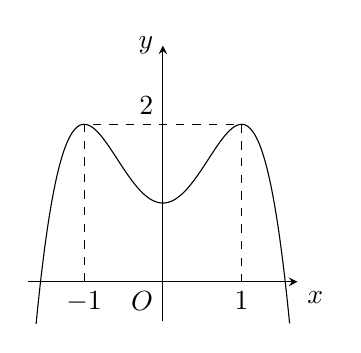
\begin{tikzpicture}[x=1cm,y=1cm,scale=1,>=stealth]
			\def\aa{-1} \def\bb{2} \def\cc{1}
			\draw[->] (-1.71,0)--(1.71,0)node[below right]{$x$};
			\draw[->] (0,-0.5)--(0,3)node[left]{$y$};
			\fill (0,0)node[below left]{$O$} (-1,0)node[below]{$-1$} (1,0)node[below]{$1$} (0,2)node[above left]{$2$};
			\draw[black,samples=150,smooth,domain=-1.61:1.61] plot(\x,{\aa*(\x)^4+\bb*(\x)^2+\cc});
			\draw[dashed] (-1,0)|-(0,2)-|(1,0);
		\end{tikzpicture}}
	\loigiai{
		Dựa vào đồ thị hàm số ta thấy $\lim\limits_{x\to +\infty}y=-\infty$.\\
		Trong bốn hàm số ở bốn phương án, chỉ có hàm số $y=-x^4+2x^2+1$ phù hợp.
	}
\end{ex}

\begin{ex}%[2D1N5-7]
	Tâm đối xứng của đồ thị hàm số $y=\dfrac{x^2-3x}{x-1}$  có tọa độ là
	\choice
	{\True $(1;-1)$}
	{$(-1;1)$}
	{$(1;-2)$}
	{$(-1;-2)$}
	\loigiai{
		Ta có $y=\dfrac{x^2-3x}{x-1}=x-2-\dfrac{2}{x-1}$.\\
		Khi đó đồ thị hàm số có đường tiệm cận đứng $x=1$ và đường tiệm cận xiên $y=x-2$.\\
		Khi đó giao điểm của hai đường tiệm cận là $(1;-1)$.\\
		Vậy tâm đối xứng của đồ thị hàm số là $(1;-1)$.
	}
\end{ex}

\begin{ex}%[2D1H5-1]
	Hàm số nào dưới đây có bảng biến thiên như sau
	\begin{center}
		
\begin{tikzpicture}
			\tkzTabInit[nocadre=false,lgt=1.2,espcl=2.5,deltacl=0.6]
			{$x$ /0.6, $y'$ /0.6, $y$ /2.5}
			{$-\infty$,$-1$,$1$,$+\infty$}
			\tkzTabLine{,+,$0$,-,$0$,+,}
			\tkzTabVar{-/$-\infty$,+/$2$,-/$-2$,+/$+\infty$}
		\end{tikzpicture}
	\end{center}
	\choice
	{$y=x^4-2x^2$}
	{$y=-x^3+3x$}
	{$y=-x^4+2x^2$}
	{\True $y=x^3-3x$}
	\loigiai{
		Hàm số có bảng biến thiên như trên, trong 4 đáp án đã cho phải là hàm bậc ba với $a>0$.}
\end{ex}

\begin{ex}%[Dự án 2025_K12_TL TV]%[Phạm Thị Thanh Thuỷ]%[2D1V5-8]
	Một vật chuyển động có đồ thị của hàm quãng đường $s(t)$, hàm vật tốc $v(t)$ và hàm gia tốc $a(t)$ theo thời gian $t$ được mô tả ở hình dưới đây. Khẳng định nào dưới đây \textbf{đúng}?
	\begin{center}
		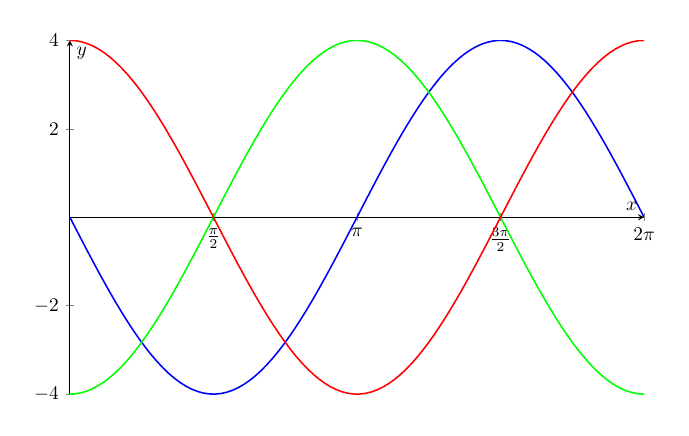
\begin{tikzpicture}[scale=0.7]
			\begin{axis}[
					domain=0:2*pi, % đoạn [0; 2pi]
					samples=100, % số lượng điểm lấy mẫu để vẽ đồ thị
					xlabel={$x$}, % nhãn trục x
					ylabel={$y$}, % nhãn trục y
					axis lines=middle, % vẽ trục tọa độ ở giữa
					%grid=major, % hiện đường lưới
					width=12cm, % chiều rộng đồ thị
					height=8cm, % chiều cao đồ thị
					xmin=0, xmax=2*pi, % giới hạn trục x
					ymin=-4, ymax=4, % giới hạn trục y
					xtick={0, pi/2, pi, 3*pi/2, 2*pi}, % các giá trị đánh dấu trên trục x
					xticklabels={$0$, $\frac{\pi}{2}$, $\pi$, $\frac{3\pi}{2}$, $2\pi$} % nhãn trục x
				]
				\addplot[
					color=blue, % màu của đồ thị
					thick % độ dày của đường đồ thị
				]
				{-4*sin(deg(x))}; % hàm số y = 4sin(x)
				\addplot[
					color=green, % màu của đồ thị
					thick % độ dày của đường đồ thị
				]
				{-4*cos(deg(x))}; % hàm số y = 4cos(x)
				\addplot[
					color=red, % màu của đồ thị
					thick % độ dày của đường đồ thị
				]
				{4*cos(deg(x))}; % hàm số y = 4sin(x)
			\end{axis}
		\end{tikzpicture}
	\end{center}
	\choice
	{\True $s(\pi)<v(\pi)<a(\pi)$}
	{$a(\pi)<v(\pi)<s(\pi)$}
	{$s(\pi)<a(\pi)<v(\pi)$}
	{$v(\pi)<a(\pi)<s(\pi)$}
	\loigiai{
		Ta có $s'(t)=v(t)$ và $v'(t)=a(t)$.\\
		Suy ra tại các điểm $t$ làm $s(t)$ đạt cực đại và cực tiểu thì $v(t)=0$, tại các điểm $t$ làm $v(t)$ đạt cực đại và cực tiểu thì $a(t)=0$.\\
		Mặt khác, tại thời điểm ban đầu $t = 0$ thì vật đang ở vị trí biên dương và sẽ dịch chuyển về vị trí cân bằng.\\
		Do đó, đường màu đỏ là $s(t)$, xanh dương là $v(t)$ còn xanh lá là $a(t)$.\\
		Từ đồ thị ta thấy
		\[s(\pi)=-4, v(\pi)=0, a(\pi)=4\Rightarrow s(\pi)<v(\pi)<a(\pi).\]
	}
\end{ex}

\begin{ex}%[KNTT]giảng 12 New-4in1, Toàn Phan]%[2D1H5-8]KNTT
	Khi bỏ qua sức cản của không khí, độ cao (mét) của một vật được phóng thẳng đứng lên trên từ điểm cách mặt đất $2$ m với vận tốc ban đầu $24{,}5$ m/s là $h(t)=2+24{,}5t-4{,}9t^2$ (theo Vật lí đại cương, NXB Giáo dục Việt Nam, $2016$). Tìm vận tốc của vật sau $2$ giây.
	\choice
	{\True $4{,}9$}
	{$2{,}4$}
	{$3{,}5$}
	{$5{,}2$}
	\loigiai{
	Theo ý nghĩa cơ học của đạo hàm, vận tốc của vật là $v=h'(t)=24{,}5-9{,}8t$ m/s.\\
	Do đó, vận tốc của vật sau $2$ giây là $v(2)=24{,}5-9{,}8\cdot 2=4{,}9$ m/s.
	}
\end{ex}

\begin{ex}%[2D1H5-8]
	Khi bỏ qua sức cản của không khí, độ cao (mét) của một vật được phóng thẳng đứng lên trên từ điểm cách mặt đất $2$ m với vận tốc ban đầu $24{,}5$ m/s là $h(t)=2+24{,}5t-4{,}9t^2$ (theo Vật lí đại cương, NXB Giáo dục Việt Nam, $2016$).
	Vật đạt độ cao lớn nhất là bao nhiêu (làm tròn đến hàng phần nghìn)?
	\choice
	{$h(2{,}5)=32{,}6$}
	{\True $h(2{,}5)=32{,}625$}
	{$h(2{,}5)=32{,}624$}
	{$h(2{,}5)=32{,}63$}
	\loigiai{
	Vì $h(t)$ là hàm số bậc hai có hệ số $a=-4{,}9< 0$ nên $h(t)$ đạt giá trị lớn nhất tại $t=-\dfrac{b}{2a}=\dfrac{24{,}5}{2\cdot 4{,}9}=2{,}5$ (giây). Khi đó, độ cao lớn nhất của vật là $h(2{,}5)=32{,}625$ m.
	}
\end{ex}

\begin{ex}%[2-H2B1-SO-2-2425]%[VN-MT-7, Trần Thị Hồng]%[1]%[2H2N1-1]
	Cho hình hộp chữ nhật $ABCD.A'B'C'D'$. Khi đó, vectơ bằng vectơ $\overrightarrow{AB}$ là
	\choice
	{\True$\overrightarrow{D'C'}$}
	{$\overrightarrow{BA}$}
	{$\overrightarrow{CD}$}
	{$\overrightarrow{B'A'}$}
	\loigiai{
		\begin{center}
			\begin{tikzpicture}[scale=.7, font=\footnotesize, line join=round, line cap=round, >=stealth]
				\def\bc{4} % cạnh BC
				\def\ba{2} % cạnh BA
				\def\gocB{35} % góc B của đáy
				\path (0,0) coordinate (A')
				(\gocB:\ba) coordinate (B')
				(\bc,0) coordinate (D')
				($(D')-( A')+(B')$) coordinate (C')
				($(B')+(90:\bc-1)$) coordinate (B)
				($(A')-(B')+(B)$) coordinate (A)
				($(D')-(B')+(B)$) coordinate (D)
				($(C')-(B')+(B)$) coordinate (C);
				\draw (A)--( A')--( D')--( C')--(C)--(B)--(A)--(D)--(C) (D')--(D);
				\draw[dashed] (B)--(B')--( C') (B')--( A');
				\foreach \x/\g in {A/180,B/90,C/90,D/90,A'/180,B'/150,C'/0,D'/-30} \fill (\x) circle(1pt)+(\g:0.3)node{$\x$};
			\end{tikzpicture}
		\end{center}
		Ta có $\overrightarrow{AB}=\overrightarrow{D'C'}$ vì chúng cùng hướng và có cùng độ dài.}
\end{ex}

\begin{ex}%[2-H2B1-SO-2-2425]%[VN-MT-7, Trần Thị Hồng]%[1]%[2H2N1-2]
	Cho hình hộp $ ABCD.A'B'C'D'$. Trong các khẳng định dưới đây, đâu là khẳng định đúng?
	\choice
	{$\overrightarrow{AB}+\overrightarrow{AC}+\overrightarrow{AD}=\overrightarrow{AC'}$}
	{\True$\overrightarrow{AB}+\overrightarrow{AA'}+\overrightarrow{AD}=\overrightarrow{AC'}$}
	{$\overrightarrow{AB}+\overrightarrow{AA'}+\overrightarrow{AD}=\overrightarrow{AC}$}
	{$\overrightarrow{AB}+\overrightarrow{AA'}+\overrightarrow{AD}=\overrightarrow{0}$}
	\loigiai{
		\begin{center}
			\begin{tikzpicture}[scale=.7, font=\footnotesize, line join=round, line cap=round, >=stealth]
				\def\bc{4} % cạnh BC
				\def\ba{2} % cạnh BA
				\def\gocB{35} % góc B của đáy
				\path (0,0) coordinate (A')
				(\gocB:\ba) coordinate (B')
				(\bc,0) coordinate(D')
				($(D')-( A')+(B')$) coordinate (C')
				($(B')+(80:\bc-1)$) coordinate (B)
				($(A')-(B')+(B)$) coordinate (A)
				($(D')-(B')+(B)$) coordinate (D)
				($(C')-(B')+(B)$) coordinate (C);
				\draw (A)--( A')--( D')--( C')--(C)--(B)--(A)--(D)--(C) (D')--(D);
				\draw[dashed] (B)--(B')--( C') (B')--( A');
				\foreach \x/\g in {A/180,B/90,C/90,D/90,A'/180,B'/150,C'/0,D'/-30}\fill (\x) circle(1pt)+(\g:0.3)node{$\x$};
			\end{tikzpicture}
		\end{center}
		Xét hình hộp $ABCD.A'B'C'D'$ ta có $\overrightarrow{AB}+\overrightarrow{AA'}+\overrightarrow{AD}=\overrightarrow{AC'}$.}
\end{ex}

\begin{ex}%[Mức độ 1]%[BG - 12 New - 4in1, Paul Hieu Nguyen]%[2H2N1-3]
	Trong không gian, khẳng định nào sau đây là khẳng định \textbf{đúng} với mọi $\overrightarrow{u}$ và $\overrightarrow{v}$ khác $\overrightarrow{0}$?
	\choice
	{\True $\overrightarrow{u}\cdot\overrightarrow{v}=\left| \overrightarrow{u} \right|\cdot\left| \overrightarrow{v} \right|\cdot\cos{\left(\overrightarrow{u}, \overrightarrow{v}\right)}$}
	{$\overrightarrow{u}\cdot\overrightarrow{v}=\left| \overrightarrow{u} \right|\cdot\left| \overrightarrow{v} \right|\cdot\sin{\left(\overrightarrow{u}, \overrightarrow{v}\right)}$}
	{$\overrightarrow{u}\cdot\overrightarrow{v}=\left| \overrightarrow{u} \right|\cdot\left| \overrightarrow{v} \right|\cdot\tan{\left(\overrightarrow{u}, \overrightarrow{v}\right)}$}
	{$\overrightarrow{u}\cdot\overrightarrow{v}=\left| \overrightarrow{u} \right|\cdot\left| \overrightarrow{v} \right|$}
	\loigiai{
		Theo định nghĩa tích vô hướng, ta có $\overrightarrow{u}\cdot\overrightarrow{v}=\left| \overrightarrow{u} \right|\cdot\left| \overrightarrow{v} \right|\cdot\cos{\left(\overrightarrow{u}, \overrightarrow{v}\right)}$.
	}
\end{ex}

\begin{ex}%[Đề chuẩn hóa- Kiểm tra chương 2]%[Nguyễn Thành Nhân]%[2H2H1-2]
	Cho tứ diện $ABCD$. Gọi $M$, $N$ theo thứ tự là trung điểm $AB$ và $CD$. Tìm khẳng định đúng trong các khẳng định sau.
	\choice
	{$\overrightarrow{MC}+\overrightarrow{MD}+\overrightarrow{NA}+\overrightarrow{NB}=4\overrightarrow{MN}$}
	{\True $\overrightarrow{AC}+\overrightarrow{BD}=2\overrightarrow{MN}$}
	{$\overrightarrow{AD}+\overrightarrow{BC}=\overrightarrow{MN}$}
	{$\overrightarrow{AC}-\overrightarrow{BD}=\overrightarrow{MN}$}
	\loigiai{
		\immini{Ta có \allowdisplaybreaks
			\begin{eqnarray*}
				\overrightarrow{AC}+\overrightarrow{BD}&=&\overrightarrow{AM}+\overrightarrow{MC}+\overrightarrow{BM}+\overrightarrow{MD}\\
				&=&\left(\overrightarrow{AM}+\overrightarrow{BM}\right)+\left(\overrightarrow{MC}+\overrightarrow{MD}\right)\\
				&=&\overrightarrow{0}+2\overrightarrow{MN}\quad (\text{do }M,\,N \,\text{lần lượt là trung điểm của }AB,\, CD).\\
				&=& 2\overrightarrow{MN}.
			\end{eqnarray*}
		}
		{
			\begin{tikzpicture}[scale=0.8, font=\footnotesize, line join=round, line cap=round, >=stealth]
				\coordinate (B) at (0,0);
				\coordinate (C) at (-30:2);
				\coordinate (D) at (0:4);
				\coordinate (A) at (75:3);
				\coordinate (M) at ($(A)!0.5!(B)$);
				\coordinate (N) at ($(C)!0.5!(D)$);
				\draw (A)--(B)--(C)--(D)--(A)--(C);
				\draw[dashed] (B)--(D) (M)--(N);
				\foreach \i/\p in{A/above,B/left,C/below,D/right,M/above left,N/below right}
				\fill[black] (\i) circle(1pt) node[\p]{$\i$};
			\end{tikzpicture}
		}
		\noindent
		Vậy mệnh đề đúng là $\overrightarrow{AC}+\overrightarrow{BD}=2\overrightarrow{MN}$.
	}
\end{ex}

\begin{ex}%[Mức độ 2]%[BG - 12 New - 4in1, Paul Hieu Nguyen]%[2H2H1-3]
	Cho hình lập phương $ABCD.A'B'C'D'$ cạnh $a$. Tính $\overrightarrow{AD}\cdot\overrightarrow{A'C'}$ theo $a$.
	\choice
	{$\overrightarrow{AD}\cdot\overrightarrow{A'C'}=0$}
	{$\overrightarrow{AD}\cdot\overrightarrow{A'C'}=\dfrac{a^2}{2}$}
	{$\overrightarrow{AD}\cdot\overrightarrow{A'C'}=\dfrac{a^2\sqrt{2}}{2}$}
	{\True $\overrightarrow{AD}\cdot\overrightarrow{A'C'}=a^2$}
	\loigiai{
		\immini
		{
			Ta có
			$\overrightarrow{AD}\cdot\overrightarrow{A'C'}=\overrightarrow{AD}\cdot\overrightarrow{AC}=AD\cdot AC\cdot\cos \widehat{CAD}=a\cdot a\sqrt{2}\cdot\dfrac{\sqrt{2}}{2}=a^2.$
		}
		{
			\begin{tikzpicture}[line join=round, line cap = round, >=stealth, scale=.7,font=\footnotesize,transform shape]
				\foreach \x/\y/\z/\g in
					{
						0/0/B/-135, 1.8/1/A/160, 4.8/1/D/0, 3/0/C/-45,
						0/3/B'/180, 1.8/4/A'/90, 4.8/4/D'/45, 3/3/C'/90
					}
				\draw[fill=black] (\x,\y) circle(1pt) coordinate (\z) ($(\z)+(\g:3.5mm)$) node{$\z$};
				\draw (D')--(C')--(B')--(A')--(D')--(D) (B')--(B)--(C)--(D) (A')--(C')--(C);
				\draw[dashed] (A')--(A)--(B) (A)--(D) (A)--(C);
			\end{tikzpicture}
		}
	}
\end{ex}

\begin{ex}%[2H2H1-1]
	Cho ba vectơ $\vec{a}, \vec{b}, \vec{c}$ không đồng phẳng. Xét các vectơ $\vec{x}=2\vec{a}+\vec{b}; \vec{y}=\vec{a}-\vec{b}-\vec{c}; \vec{z}=-3\vec{b}-2\vec{c}$. Chọn khẳng định đúng?
	\choice
	{\True Ba vectơ $\vec{x}; \vec{y}; \vec{z}$ đồng phẳng}
	{Hai vectơ $\vec{x}; \vec{a}$ cùng phương}
	{Hai vectơ $\vec{x}; \vec{b}$ cùng phương}
	{Ba vectơ $\vec{x}; \vec{y}; \vec{z}$ đôi một cùng phương}
	\loigiai{
		Ta có $\vec{y}=\dfrac{1}{2}(\vec{x}+\vec{z})$ nên ba vectơ $\vec{x}; \vec{y}; \vec{z}$ đồng phẳng.}
\end{ex}

\begin{ex}%[2H2V1-3]
	Cho tứ diện $ABCD$  có trọng tâm  $G$. Chọn khẳng định đúng.
	\choice
	{$AB^2 + AC^2 + AD^2 + BC^2 + BD^2 + CD^2 = 3\left(GA^2 + GB^2 + GC^2 + GD^2\right)$}
	{\True $AB^2 + AC^2 + AD^2 + BC^2 + BD^2 + CD^2 = 4\left(GA^2 + GB^2 + GC^2 + GD^2\right)$}
	{$AB^2 + AC^2 + AD^2 + BC^2 + BD^2 + CD^2 = 6\left(GA^2 + GB^2 + GC^2 + GD^2\right)$}
	{$AB^2 + AC^2 + AD^2 + BC^2 + BD^2 + CD^2 = 2\left(GA^2 + GB^2 + GC^2 + GD^2\right)$}
	\loigiai{
		\begin{center}
			\begin{tikzpicture}[scale=1,>=stealth, font=\footnotesize, line join=round, line cap=round]
				\def\a{4}
				\path 	(0:0) coordinate (B)
				++(0:\a) coordinate (D)
				++(-150:.8*\a) coordinate (C)
				($(B)+(70:\a)$) coordinate (A)
				($(A)!.5!(B)$) coordinate (I)
				($(C)!.5!(D)$) coordinate (J)
				($(I)!.5!(J)$) coordinate (G)
				;

				\draw[dashed] (B)--(D) (G)--(A) (G)--(B) (G)--(C)(G)--(D) (I)--(J);
				\draw (B)--(A)--(D) (A)--(C)
				(B)--(C)--(D);
				\foreach \x/\g in {A/90,B/180,C/-45,D/0,G/30,I/150,J/-60}
				\fill[black] 	(\x) circle (1pt)
				($(\g:3mm)+(\x)$) node {$\x$};
				%Hình chóp S.ABC có SA vuông góc đáy
			\end{tikzpicture}
		\end{center}
		Ta có

		$ AB^2 + AC^2 + AD^2 + BC^2 + BD^2 + CD^2$\\
		$ =\left(\overrightarrow{AG} + \overrightarrow{GB}\right)^2
			+ \left(\overrightarrow{AG} + \overrightarrow{GC}\right)^2
			+ \left(\overrightarrow{AG} + \overrightarrow{GD}\right)^2
			+ \left(\overrightarrow{BG} + \overrightarrow{GC}\right)^2
			+ \left(\overrightarrow{BG} + \overrightarrow{GD}\right)^2
			+ \left(\overrightarrow{BG} + \overrightarrow{GD}\right)^2$
		$ = 3AG^2 + 3BG^2 + 3CG^2 + 3DG^2 +$

		$  + 2\left(\overrightarrow{AG}\cdot\overrightarrow{GB}
			+ \overrightarrow{AG} \cdot \overrightarrow{GC}
			+ \overrightarrow{AG} \cdot \overrightarrow{GD}
			+ \overrightarrow{BG} \cdot \overrightarrow{GC}
			+ \overrightarrow{BG} \cdot \overrightarrow{GD}
			+ \overrightarrow{BG} \cdot \overrightarrow{GD}\right)$. $\qquad (1)$\\
		Lại có

		$\overrightarrow{GA} + \overrightarrow{GB} + \overrightarrow{GC} +\overrightarrow{GD} = \overrightarrow{0}$\\
		$\Leftrightarrow\left(GA^2 + GB^2 + GC^2 + GD^2\right)=$

		$=2\left(\overrightarrow{AG}\cdot\overrightarrow{GB}
			+ \overrightarrow{AG} \cdot \overrightarrow{GC}
			+ \overrightarrow{AG} \cdot \overrightarrow{GD}
			+ \overrightarrow{BG} \cdot \overrightarrow{GC}
			+ \overrightarrow{BG} \cdot \overrightarrow{GD}
			+ \overrightarrow{BG} \cdot \overrightarrow{GD}\right)$. $\qquad (2)$\\
		Từ $(1)$ và $(2)$ ta có điều phải chứng minh.

	}
\end{ex}

\begin{ex}%[2-H2B3-SO-8-2425]%[VN-MT-7, Phan Hoàng Anh]%[2H2N2-2]
	Trong không gian $Oxyz$, cho $2$ điểm $A(1;2;3)$, $B(-1;1;-1)$. Gọi $I$ là trung điểm của đoạn thẳng $AB$, tọa độ điểm $I$ là
	\choice
	{$I\left(0;\dfrac{3}{2};-1\right)$}
	{$I(0;3;2)$}
	{$I\left(2;\dfrac{5}{2};5\right)$}
	{\True $I\left(0;\dfrac{3}{2};1\right)$}
	\loigiai{Gọi $I\left(x_0;y_0;z_0\right)$ là trung điểm của đoạn $AB$.\\
		Ta có $\heva{&x_0=\dfrac{1+(-1)}{2}=0\\&y_0=\dfrac{2+1}{2}=\dfrac{3}{2}\\&z_0=\dfrac{3+(-1)}{2}=1}\Rightarrow I\left(0;\dfrac{3}{2};1\right)$.}
\end{ex}

\begin{ex}%[2H2N2-1]
	Khối cầu có bán kính $R$ thì thể tích được tính theo công thức
	\choice
	{\True $V=\dfrac{4}{3}\pi R^3$}
	{$V=\dfrac{1}{3}\pi R^3$}
	{$V=4\pi R^3$}
	{$V=\dfrac{4}{3}\pi R^2$}
	\loigiai{
		Khối cầu có bán kính $R$ thì thể tích được tính theo công thức\\
		\centerline{$V=\dfrac{4}{3}\pi R^3$.}
	}
\end{ex}

\begin{ex}%[VN-MT-7, Lê Minh Thiện Anh]%[2H2N2-4]
	Trong không gian $Oxyz$, cho tam giác $ABC$ có $A(3;-2;5)$, $B(-2;1;-3)$, $C(5;1;1)$. Tìm tọa độ trọng tâm $G$ của tam giác $ABC$.
	\choice
	{$G(-2;0;1)$}
	{$G(2;1;-1)$}
	{\True $G(2;0;1)$}
	{$G(2;0;-1)$}
	\loigiai{
		Ta có $\heva{&x_G=\dfrac{x_A+x_B+x_C}{3}=\dfrac{3+(-2)+5}{3}=2\\&y_G=\dfrac{y_A+y_B+y_C}{3}=\dfrac{(-2)+1+1}{3}=0\\&z_G=\dfrac{z_A+z_B+z_C}{3}=\dfrac{5+(-3)+1}{3}=1.}$\\
		Vậy $G(2;0;1)$.
	}
\end{ex}

\begin{ex}%[2H2H2-1]
	Trong không gian với hệ tọa độ $Oxyz$, cho $3$ vectơ $\vec{a}=\left(2;-5;3\right)$, $\vec{b}=\left(0;2;-1\right)$, $\vec{c}=\left(1;7;2\right)$. Tìm tọa độ $\vec{d}=\vec{a}-4\vec{b}-2\vec{c}$.
	\choice
	{\True $\left(0;-27;3\right)$}
	{$\left(1;2;-7\right)$}
	{$\left(0;27;3\right)$}
	{$\left(0;27;-3\right)$}
	\loigiai{
		Ta có $\vec{a}=\left(2;-5;3\right),4\vec{b}=\left(0;8;-4\right),2\vec{c}=\left(2;14;4\right)$.\\
		Suy ra $\vec{d}=\left(2-0-2;-5-8-14;3-(-4)-4\right)=\left(0;-27;3\right)$.
	}
\end{ex}

\begin{ex}%[ID6]%[CTST-Lop12-Ontapcuoihocki1-De4]%[Bùi Lương Phúc]%[2H2H2-4]
	Trong không gian tọa độ $Oxyz$, cho $A(1; 2; 3)$, $B(-1; 1; 2)$, $C(2; 1; 1)$. Tính côsin của góc tạo bởi $\overrightarrow{AB}$ và $\overrightarrow{AC}$.
	\choice
	{$\dfrac{1}{2}$}
	{$\dfrac{1}{3}$}
	{\True $\dfrac{1}{6}$}
	{$\dfrac{1}{4}$}
	\loigiai
	{
		Ta có $\overrightarrow{AB} = (-2; -1; -1), \quad \overrightarrow{AC} = (1; -1; -2)$.\\
		$\overrightarrow{AB} \cdot \overrightarrow{AC} = (-2)(1) + (-3)(-3) + (-1)(-2) = -2 + 9 + 2 = 9$.\\
		$ \left|\overrightarrow{AB}\right| = \sqrt{(-2)^2 + (-3)^2 + (-1)^2} = \sqrt{14}, \left|\overrightarrow{AC}\right| = \sqrt{1^2 + (-3)^2 + (-2)^2} = \sqrt{14}$.\\
		Gọi góc tạo bởi $\overrightarrow{AB}$ và $\overrightarrow{AC}$ là $\theta$ thì\\
		\[
			\cos \theta = \frac{\overrightarrow{AB} \cdot \overrightarrow{AC}}{\left|\overrightarrow{AB}\right| \left|\overrightarrow{AC}\right|} = \frac{9}{14}.
		\]
	}
\end{ex}

\begin{ex}%[2H2V2-6]
	Cho hình chóp $S.ABCD$ đáy là hình thang vuông tại $A$ và $D$, $SA\perp(ABCD)$. Góc giữa $SB$ và mặt phẳng đáy bằng $45^{\circ}$, $E$ là trung điểm của $SD$, $AB=2a$, $AD=DC=a$. Gọi $G$ là trọng tâm của tam giác $ACE$. Độ dài $BG$ bằng
	\choice
	{$BG=\dfrac{a\sqrt{89}}{6}$}
	{\True $BG=\dfrac{a\sqrt{113}}{6}$}
	{$BG=\dfrac{a\sqrt{89}}{2}$}
	{$BG=\dfrac{a\sqrt{89}}{3}$}
	\loigiai{
	\begin{center}
		\begin{tikzpicture}[>=stealth,line join=round,line cap=round]
			\draw[line width=1pt,black,scale=2.5] (0,0)coordinate(A)  (-120:1)coordinate(D)--($(1,0)-(A)+(D)$)coordinate(C)--(2,0)coordinate(B) (D)--($(A)+(90:1)$)coordinate(S)--(C) (S)--(B);
			\draw[dashed,line width=1pt,black,scale=2.5] (D)--(A)--(B) (S)--(A);
			\path[scale=2.5] pic[angle radius=5,draw=blue,angle eccentricity=1.5] {right angle = B--A--S};
			\draw[->, red] (B)--($1.25*(B)-0.25*(A)$)coordinate(X)node[above]{$x$};
			\draw[->, red] (D)--($1.25*(D)-0.25*(A)$)coordinate(Y)node[left]{$y$};
			\draw[->, red] (S)--($1.25*(S)-0.25*(A)$)coordinate(Z)node[right]{$z$};
			\foreach \diem/\vitrin in {S/left,A/left,D/left,C/below right,B/above} \fill (\diem)circle(1.5pt)node[\vitrin]{$\diem$};
		\end{tikzpicture}\end{center}
	Hình chiếu của $SB$ trên mặt phẳng $(ABCD)$ là $AB$, suy ra góc giữa $SB$ và mặt đáy là góc giữa $SB$ và $AB$ và bằng góc $\widehat{SBA}=45^{\circ}$.\\
	Tam giác $SAB$ vuông cân tại $A$ nên $SA=2a$.\\
	Chọn hệ trục tọa độ như hình vẽ ta có $A(0;0;0)$, $B(0;2a;0)$, $C(a;a;0)$, $D(a;0;0)$, $S(0;0;2a)$, $E(\dfrac{a}{2};0;a)$.\\
	Gọi $G$ là trọng tâm của tam giác $ACE$ nên $G\left(\dfrac{a}{2};\dfrac{a}{3};\dfrac{a}{3}\right)$.\\
	Độ dài $BG$ là: $BG=\sqrt{\left(\dfrac{a}{2}-0\right)^2+\left(\dfrac{a}{3}-2a\right)^2+\left(\dfrac{a}{3}-0\right)^2}=\dfrac{a\sqrt{113}}{6}$.
	}
\end{ex}

\begin{ex}%[12-MH-1-MH2025]%[MH-2025, Mã/Tên TV biên soạn]%[2D3N1-1]
	Xét mẫu số liệu ghép nhóm có tứ phân vị thứ nhất, tứ phân vị thứ hai, tứ phân vị thứ ba lần lượt là $Q_1$, $Q_2$ và $Q_3$. Khoảng tứ phân vị của mẫu số liệu ghép nhóm đó bằng
	\choice
	{$Q_2 - Q_1$}
	{$Q_3 - Q_2$}
	{\True $Q_3 - Q_1$}
	{$Q_3 - 2Q_2 + Q_1$}
	\loigiai{Khoảng tứ phân vị của mẫu số liệu ghép nhóm đó là $Q_3 - Q_1$.
	}
\end{ex}

\begin{ex}%[2D3H1-2]
	Thời gian và số ngày tập thể dục của bác T và bác H trong một tháng (30 ngày) được thống kê theo bảng dưới đây
	\begin{longtable}[c]
		{|c|c|c|c|}
		\hline
		Thời gian tập (phút)  & $[15;20)$ & $[25;30)$ & $[30;35)$ \\
		\hline
		Số ngày tập của bác T & $10$      & $15$      & $5$       \\
		\hline
		Số ngày tập của bác H & $9$       & $21$      & $0$       \\
		\hline
	\end{longtable}
	\noindent Mệnh đề nào sau đây đúng?
	\choice
	{Khoảng biến thiên thời gian tập của bác T bằng $10$}
	{Khoảng biến thiên thời gian tập của bác H bằng $20$}
	{\True Độ phân tán thời gian tập của bác Tcao hơn độ phân tán thời gian tập của bác H}
	{Độ phân tán thời gian tập của bác T thấp hơn độ phân tán thời gian tập của bác H}
	\loigiai{
		Khoảng biến thiên của mẫu số liệu ghép nhóm về thời gian tập của bác T là $35$ – $15=20$ (phút).\\
		Khoảng biến thiên của mẫu số liệu ghép nhóm về thời gian tập của bác H là $30$ – $15=15$ (phút).\\
		Do đó căn cứ theo khoảng biến thiên thì thời gian tập của bác T có độ phân tán lớn hơn.}
\end{ex}

\begin{ex}%[2-D3B1-SO-3-2425]%[VN-MT-7-NguyenVanMinhHieu]%[2D3H1-3]
	Người ta tiến hành phỏng vấn $40$ người về một mẫu áo khoác. Người điều tra yêu cầu cho điểm mẫu áo đó theo thang điểm là $100$. Kết quả được trình bày trong bảng ghép nhóm sau:
	\begin{center}
		\begin{tabular}{|c|c|c|c|c|c|c|}
			\hline
			Nhóm   & $[50;60)$ & $[60;70)$ & $[70;80)$ & $[80;90)$ & $[90;100)$ &        \\
			\hline
			Tần số & $4$       & $5$       & $23$      & $6$       & $2$        & $n=40$ \\
			\hline
		\end{tabular}
	\end{center}
	Tìm khoảng tứ phân vị của dãy số liệu trên (làm tròn đến hàng đơn vị).
	\choice
	{$11$}
	{\True $9$}
	{$15$}
	{$10$}
	\loigiai{
	Gọi $x_1$, $x_2$, $\ldots$, $x_{40}$ lần lượt là điểm mẫu áo khoác theo thứ tự không giảm.\\
	Tứ phân vị thứ nhất của dãy số liệu là $\dfrac{1}{2}(x_{10}+x_{11})$ thuộc nhóm $[70;80)$ nên tứ phân vị thứ nhất của mẫu số liệu là
	\[Q_1=70+\dfrac{\dfrac{40}{4}-9}{23}\cdot(80-70) \approx 70{,}4.\]
	Tứ phân vị thứ ba của dãy số liệu là $\dfrac{1}{2}(x_{30}+x_{31})$ thuộc nhóm $[70;80)$ nên tứ phân vị thứ ba của mẫu số liệu là
	\[Q_3=70+\dfrac{\dfrac{3\cdot 40}{4}-9}{23}\cdot(80-70)\approx 79{,}1.\]
	Vậy khoảng tứ phân vị của mẫu số liệu trên là $\Delta_Q=Q_3-Q_1 \approx 8{,}7$.
	}
\end{ex}

\begin{ex}%[2-D3B1-SO-3-2425]%[VN-MT-7-NguyenVanMinhHieu]%[2D3H1-4]
	Tổng hợp tiền lương tháng của một số nhân viên văn phòng được ghi lại như sau (đơn vị: triệu đồng)
	\begin{center}
		\begin{tabular}{|c|c|c|c|c|}
			\hline
			Lương tháng (triệu đồng) & $[6;8)$ & $[8;10)$ & $[10;12)$ & $[12;14)$ \\
			\hline
			Số nhân viên             & $3$     & $6$      & $8$       & $7$       \\
			\hline
		\end{tabular}
	\end{center}
	Giá trị nào sau đây là giá trị ngoại lệ của mẫu số liệu trên
	\choice
	{\True $3$}
	{$9$}
	{$15$}
	{$10$}
	\loigiai{
	Gọi $x_1$, $x_2$, $\ldots$, $x_{24}$ lần lượt là lương tháng của mỗi nhân viên được xếp theo thứ tự không giảm.\\
	Tứ phân vị thứ nhất của mẫu số liệu là $\dfrac{1}{2}(x_6+x_7)$.\\
	Do $x_6$, $x_7 \in [8;10)$ nên tứ phân vị thứ nhất của mẫu số liệu ghép nhóm là
	\[Q_1=8+\dfrac{\dfrac{24}{4}-3}{6}\cdot(10-8)=9\]
	Tứ phân vị thứ ba của mẫu số liệu là $\dfrac{1}{2}(x_{18}+x_{19})$.\\
	Do $x_{18}$, $x_{19} \in [12;14)$ nên tứ phân vị thứ ba của mẫu số liệu ghép nhóm là
	\[Q_3=12+\dfrac{\dfrac{3\cdot 24}{4}-17}{7}\cdot(14-12)=\dfrac{86}{7}\approx 12{,}3\]
	Khoảng tứ phân vị là $\Delta_Q=Q_3-Q_1=\dfrac{86}{7}-9=\dfrac{23}{7}\approx 3{,}3$.\\
	Ta có $[Q_1-1{,}5\Delta_Q;Q_3+1{,}5\Delta_Q ]\approx [4{,}07;17{,}2]$.\\
	Vậy giá trị ngoại lệ là $3$.}
\end{ex}

\begin{ex}%[2D3H2-1]%[Du-An-Ngan-Hang-Cau-Hoi-2024-K12]
	Yếu tố được dùng để đo mức độ phân tán của mẫu số liệu ghép nhóm xung quanh số trung bình của mẫu số liệu là
	\choice
	{khoảng biến thiên}
	{khoảng tứ phân vị}
	{phương sai}
	{\True phương sai và độ lệch chuẩn}
	\loigiai{Yếu tố được dùng để đo mức độ phân tán của mẫu số liệu ghép nhóm xung quanh số trung bình của mẫu số liệu là phương sai và độ lệch chuẩn.}
\end{ex}

\begin{ex}%[2-D3B3-SO-8-2425]%[VN-MT-7, Lại Thị Hảo]%[2D3H2-2]
	Mỗi ngày bác An đều đi bộ để rèn luyện sức khỏe. Quãng đường đi bộ mỗi ngày (đơn vị: km) của bác An trong $20$ ngày được thống kê lại ở bảng sau:
	\begin{center}
		\begin{tabular}{|c|c|c|c|c|c|}
			\hline
			Quãng đường (km) & $[2{,}7; 3{,}0)$ & $[3{,}0; 3{,}3)$ & $[3{,}3; 3{,}6)$ & $[3{,}6; 3{,}9)$ & $[3{,}9; 4{,}2)$ \\
			\hline
			Số ngày          & $3$              & $6$              & $5$              & $4$              & $2$              \\
			\hline
		\end{tabular}
	\end{center}
	Phương sai của mẫu số liệu ghép nhóm là
	\choice
	{$3{,}39$}
	{$11{,}62$}
	{\True $0{,}1314$}
	{$0{,}36$}
	\loigiai{
	Ta có bảng sau:
	\begin{center}
		\begin{tabular}{|c|c|c|c|c|c|}
			\hline
			Quãng đường (km) & $[2{,}7; 3{,}0)$ & $[3{,}0; 3{,}3)$ & $[3{,}3; 3{,}6)$ & $[3{,}6; 3{,}9)$ & $[3{,}9; 4{,}2)$ \\
			\hline
			Giá trị đại diện & $2{,}85$         & $3{,}15$         & $3{,}45$         & $3{,}75$         & $4{,}05$         \\
			\hline
			Số ngày          & $3$              & $6$              & $5$              & $4$              & $2$              \\
			\hline
		\end{tabular}
	\end{center}
	Số trung bình của mẫu số liệu ghép nhóm là
	\[\overline{x}=\dfrac{3 \cdot 2{,}85+6 \cdot 3{,}15+5 \cdot 3{,}45+4 \cdot 3{,}75+2 \cdot 4{,}05}{20}=3{,}39.\]
	Phương sai của mẫu số liệu ghép nhóm là
	\[s^2=\dfrac{3 (2{,}85-3{,}39)^2+6(3{,}15-3{,}39)^2+5(3{,}45-3{,}39)^2+4(3{,}75-3{,}39)^2+2 (4{,}05-3{,}39)^2}{20}=0{,}1314.\]
	}
\end{ex}
\Closesolutionfile{ans}
\TL
\begin{bt}%[2D3H2-2]
	Mỗi ngày anh $A$ đều đi bộ để rèn luyện sức khỏe. Quãng đường đi bộ mỗi ngày (đơn vị $\mathrm{km}$) của anh A trong 20 ngày được thống kê 1ại ở bảng sau
	\begin{center}
		\begin{tabular}{|c|c|c|c|c|c|}
			\hline Quãng đường $(\mathrm{km})$ & {$[2{,}7 ; 3{,}0)$} & {$[3{,}0 ; 3{,}3)$} & {$[3{,}3 ; 3{,}6)$} & {$[3{,}6 ; 3{,}9)$} & {$[3{,}9 ; 4{,}2)$} \\
			\hline Số ngày                     & 3                   & 6                   & 5                   & 4                   & 2                   \\
			\hline
		\end{tabular}
	\end{center}
	Tính phương sai của mẫu số liệu trên (làm tròn kết quả đến hàng phần chục).
	\loigiai{Ta có bảng sau
	\begin{center}
		\begin{tabular}{|c|c|c|c|c|c|}
			\hline Quãng đường $(\mathrm{km})$ & {$[2{,}7 ; 3{,}0)$} & {$[3{,}0; 3{,}3)$} & {$[3{,}3 ; 3{,}6)$} & {$[3{,}6 ; 3{,}9)$} & {$[3{,}9 ; 4{,}2)$} \\
			\hline Giá trị đại diện            & $2{,}85$            & $3{,}15$           & $3{,}45$            & $3{,}75$            & $4{,}05$            \\
			\hline Số ngày                     & $3$                 & $6$                & $5$                 & $4$                 & $2$                 \\
			\hline
		\end{tabular}
	\end{center}
	Số trung bình của mẫu số liệu ghép nhóm là
	\[
		\overline{x}=\dfrac{3\cdot2{,}85+6\cdot3{,}15+5\cdot3{,}45+4\cdot3{,}75+2\cdot4{,}05}{20}=3{,}39.
	\]
	Phương sai của mẫu số liệu ghép nhóm là
	\[
		S^2=\dfrac{1}{20}\left[3 \cdot(2{,}85)^2+6 \cdot(3,15)^2+5 \cdot(3{,}45)^2+4 \cdot(3{,}75)^2+2 \cdot(4{,}05)^2\right]-(3{,}39)^2\approx0{,}1.
	\]
	}
\end{bt}

\begin{bt}%[SGK12-Cùng Khám Phá]%[2D1H5-8]
	Kính viễn vọng Hubble được tàu không gian Discovery đưa vào sử dụng ngày 24/4/1990. Mô hình vận tốc của tàu trong sứ mệnh này, từ lúc rời bệ phóng ($t=0$ giây) cho đến khi được tên lửa đẩy nhanh khỏi bệ tại thời điểm $t=126$ giây, được xác định bởi công thức:\\ $v(t)=0{,}001302t^3-0{,}09029t^2+23{,}61t-3{,}083$ (feet/giây) (nguồn: James Stewart, J. (2015). \textit{Calculus. Cengage Learning 8th edition,} p. 282). Tính gia tốc lớn nhất của tàu trong khoảng thời gian này (làm tròn kết quả đến hàng phần trăm).
	\loigiai{
	Gia tốc của tàu trong khoảng thời gian $t=0$ giây đến $t=126$ giây được xác định bởi công thức
	$$a(t)=v'(t)=0{,}003906t^2-0{,}18058t+23{,}61 ~(\text{ft/s}^2) ~\text{với}~ t \in [0;126].$$
	Ta có $a'(t)=0{,}007812t-0{,}18058$. \\
	$a'(t)=0 \Leftrightarrow 0{,}007812t-0{,}18058 =0 \Leftrightarrow t = \dfrac{45145}{1953}$.\\
	Ta có $a(0)=23{,}61$, $a \left( \dfrac{45145}{1953} \right) \approx 21{,}52$, $a(126) \approx 62{,}87$.\\
	Vậy gia tốc lớn nhất của tàu trong khoảng thời gian trên là $62{,87} \; (\text{ft}/s^2)$.
	}
\end{bt}

\begin{bt}%[2-H2B4-SO-12-2425 (Nguồn Đề 3 - )]%[VN-MT-7, Vũ Hồng Toàn]%[2H2V2-6]
	\immini{
		Một vật nặng có trọng lượng là $400$ N được đặt trên một khung sắt hình tròn như hình bên. Biết $ABCD$ là hình chữ nhật, mặt phẳng $(ABCD)$ song song với mặt phẳng nằm ngang. Khung sắt được móc vào điểm $S$ sao cho các đoạn dây cáp $SA$, $ SB$, $SC$, $SD$ có độ dài bằng nhau và cùng tạo với mặt phẳng $(ABCD)$ một góc bằng $45^\circ$. Chiếc cần cẩu kéo khung sắt lên theo phương thẳng đứng. Biết trọng lượng của khung sắt là $200$ N; cường độ các lực căng $\overrightarrow{F}_1$, $\overrightarrow{F}_2$, $\overrightarrow{F}_3$, $\overrightarrow{F}_4$ là bằng nhau. Tính cường độ của lực căng $\overrightarrow{F}_1$ (làm tròn đến hàng đơn vị).
	}
	{
		\begin{tikzpicture}[scale=.7,>=stealth, font=\footnotesize, line join=round, line cap=round]
			\definecolor{beaver}{rgb}{0.62, 0.51, 0.44}
			\definecolor{atomictangerine}{rgb}{1.0, 0.6, 0.4}
			\definecolor{bittersweet}{rgb}{1.0, 0.44, 0.37}
			\tikzset{day/.pic=
					{\draw[black,rounded corners=.5ex,line width=.5pt]
						(0,0) rectangle (1mm,2mm)
						(.5mm,0)--(.5mm,-.2)
						(.5mm,2mm)--(.5mm,.4);}
			}
			\def\h{6}
			\def\a{3}
			\def\b{1.5}
			\path
			(0,0) coordinate (O)
			($(O)+(0,\h)$) coordinate (S)
			($(O)+(10:\a cm and \b cm)$)coordinate (M)
			($(O)+(180:\a cm and .8*\b cm)$)coordinate (A)
			($(O)+(0:\a cm and .8*\b cm)$)coordinate (C)
			($(O)+(0,.05)+(60:\a cm and .8*\b cm)$)coordinate (B)
			($(O)+(.2,0)+(-120:\a cm and .8*\b cm)$)coordinate (D)
			;

			\draw[fill=beaver]  (M) arc (10:-190:\a cm and \b cm);
			\draw[fill=white]  (M) arc (10:-190:\a cm and .8*\b cm);
			\draw [fill=white] (M) arc (10:190:\a cm and .8*\b cm);

			\foreach \m in {0,1,2,...,11,11}{\pic[rotate=-22] at ($(A)+(.25*\m,.5*\m)$) {day};}
			\foreach \m in {0,1,2,...,13}{\pic[rotate=-15] at ($(D)+(.09*\m,.5*\m)$) {day};}
			\foreach \m in {0,1,2,...,8,9}{\pic[rotate=12] at ($(B)+(-.12,0)+(-.15*\m,.5*\m)$) {day};}
			\foreach \m in {0,1,2,...,11}{\pic[rotate=22] at ($(C)+(-.15,0)+(-.25*\m,.5*\m)$) {day};}
			\foreach \x/\y in {A/180,B/-60,C/-45,D/-90}
			\fill[black] (\x) circle (2pt) ($(\y:7mm)+(\x)$) node {$\x$};
			\fill[black] ($(S)+(0,-.22)$) circle (2pt) ($(80:6mm)+(S)$) node {$S$};

			\draw[fill=beaver] (S) circle (6pt);
			\draw[fill=white] (S) circle (4pt);

			\draw[fill=bittersweet] ($(O)+(.3*\a,0)$) arc (0:-180:.3*\a cm and .15*\b cm)-- ++(0,.3)-- ++(.6*\a,0)--cycle;
			\draw[fill=atomictangerine] ($(O)+(.3*\a,.3)$) arc (0:360:.3*\a cm and .15*\b cm);
			\foreach \i/\j [count =\k from 1] in {A/180,B/245,C/0,D/-65}{\draw[->] (S)-- ($(S)!0.6!(\i)$) coordinate(\i') node[midway, shift={(\j:5mm)}]{$\overrightarrow{F}_\k$};}
		\end{tikzpicture}
	}
	\loigiai{
		\begin{center}
			\begin{tikzpicture}[scale=1, font=\footnotesize, line join=round, line cap=round, >=stealth]
				\def\a{4.5} \def\b{2.2} \def\h{4.5} \def\g{40}
				\path
				(0,0) coordinate (A)
				(0:\a) coordinate (B)++
				(-\g:\b) coordinate (C)++(180:\a) coordinate (D)
				($(A)!.5!(C)$) coordinate (O)++ (90:\h) coordinate (S)
				;
				\draw[dashed] (S)--(B)--(A)--(C)--(B)--(D) (S)--(O);
				\draw (S)--(A)--(D)--(C)--(S)--(D);
				\foreach \i/\j [count =\k from 1] in {A/180,D/210,C/-10}{\draw[->] (S)-- ($(S)!0.65!(\i)$) coordinate(\i') node[midway, shift={(\j:4mm)}]{$\overrightarrow{F}_\k$};}
				\draw[->, dashed] (S)-- ($(S)!0.65!(B)$) coordinate(B') node[midway, shift={(250:4mm)}]{$\overrightarrow{F}_4$};
				\draw (A')--(D')--(C');
				\draw[dashed] (D')--(B')--(A')--(C')--(B');
				\draw[->, dashed] (S)--($(S)!0.65!(O)$) coordinate(O');
				\foreach \x /\g in {A/160,D/-90,C/-20,S/90,O/-90,B/30, A'/160, D'/220, C'/10, B'/40, O'/-55}
				\fill(\x) circle (1pt)($(\x)+(\g:3mm)$) node {$\x$};
			\end{tikzpicture}
		\end{center}
		Gọi $O$ là hình chiếu vuông góc của $S$ trên $(ABCD)$. Ta có $SA=SB=SC=SD$ nên các tam giác vuông $SOA$, $SOB$, $SOC$, $SOD$ bằng nhau. Suy ra $OA=OB=OC=OD$ hay $O$ là tâm hình chữ nhật $ABCD$.\\
		Gọi $A'$, $B'$, $C'$, $D'$ lần lượt là các điểm sao cho $\overrightarrow{SA'}=\overrightarrow{F}_1$, $\overrightarrow{SB'}=\overrightarrow{F}_2$, $\overrightarrow{SC'}=\overrightarrow{F}_3$ và $\overrightarrow{SD'}=\overrightarrow{F}_4$.\\
		Vì $\left|\overrightarrow{F}_1\right| = \left|\overrightarrow{F}_2\right| = \left|\overrightarrow{F}_3\right| = \left|\overrightarrow{F}_4\right|$ nên $SA'=SB'=SC'=SD'$. Do đó $S.A'B'C'D'$ là hình chóp có đáy $A'B'C'D'$ là hình chữ nhật.\\
		Gọi $O'$ là tâm hình chữ nhật $A'B'C'D'$, ta có $O'$ thuộc $SO$.\\
		Ta có
		\begin{align*}
			\overrightarrow{F}_1 + \overrightarrow{F}_2 + \overrightarrow{F}_3 + \overrightarrow{F}_4 & = \overrightarrow{SA'} + \overrightarrow{SB'} + \overrightarrow{SC'} + \overrightarrow{SD'}                           \\
			                                                                                          & = \left(\overrightarrow{SA'} + \overrightarrow{SC'}\right) + \left(\overrightarrow{SB'} + \overrightarrow{SD'}\right) \\
			                                                                                          & =4\overrightarrow{SO'}.
		\end{align*}
		Gọi $\overrightarrow{P}$ là trọng lực của vật nặng và khung sắt. Do vật và khung sắt ở vị trí cân bằng nên
		\[\overrightarrow{P} = \overrightarrow{F}_1 + \overrightarrow{F}_2 + \overrightarrow{F}_3 + \overrightarrow{F}_4 = 4\overrightarrow{SO'}.\]
		Theo giả thiết ta có $\left|\overrightarrow{P}\right|=400+200=600$ N nên $4\left|\overrightarrow{SO'}\right| =600 \Leftrightarrow SO'=150$.\\
		Lại có $\bigl(SA,(ABCD)\bigr)=\widehat{SAO}=\widehat{SA'O'}=45^\circ$.\\
		Vì $\triangle SO'A'$ vuông tại $O'$ nên $SA'=\dfrac{SO'}{\sin 45^{\circ}}=150\sqrt{2}$.\\
		Vậy cường độ của lực căng $\overrightarrow{F}_1$ là $\left|\overrightarrow{F}_1\right| = 150\sqrt{2}\approx 212$ N.
	}
\end{bt}

\begin{bt}%[2-TK-HK1-SO-10-2425]%[VN-MT-7, Nguyễn Cao Cường]%[2D1C3-6]
	Ông Vinh đang ở trong rừng để đào vàng và ông ta tìm thấy vàng ở điểm $X$ cách điểm $A$ một khoảng $3$ km . Điểm $A$ nằm trên đường bờ biển (đường bờ biển là đường thẳng). Trại của ông Vinh nằm ở vị trí $Y$ cách điểm $B$ một khoảng $3$ km. Điểm $B$ cũng thuộc đường bờ biển. Biết rằng $AB=18$ km, $AM=NB=x$ km và $AX=BY=3$ km (minh hoạ như hình vẽ sau).
	\begin{center}
		\begin{tikzpicture}[line cap=round,line join=round,>=stealth,scale=1]
			\path
			(0,0)coordinate(O)++(0:2)coordinate(A)++(0:3)coordinate(M)++(0:3.5)coordinate(N)++(0:3)coordinate(B)++(0:2)coordinate(O')
			(A)++(90:3.5)coordinate(X)
			(B)++(90:3.5)coordinate(Y)
			;
			\foreach \x/\g in{A/-90,B/-90,N/-90,X/90,M/-90,Y/90}
			\fill[black](\x) circle (1pt)
			($(\x)+(\g:3mm)$) node{\small $\x$};
			\draw (O)--(O')node[below,midway]{Bờ biển}
			(A)--(M)node[below,midway]{$x$}
			(N)--(B)node[below,midway]{$x$}
			(A)--(X)node[left,midway]{$3$ km}
			(Y)--(B)node[right,midway]{$3$ km}
			;
			\draw[dashed] (X)--(M) (N)--(Y)
			;
			\draw[<->] ($(A)+(0,-1)$)--($(B)+(0,-1)$)node[below,midway]{$18$ km}
			;
		\end{tikzpicture}
	\end{center}
	Khi đang đào vàng, ông Vinh không may bị rắn cắn, chất độc lan vào máu. Sau khi bị cắn, nồng độ chất độc trong máu tăng theo thời gian được tính theo phương trình $y=50 \log (t+2)$. Trong đó, $y$ là nồng độ, $t$ là thời gian tính bằng giờ sau khi bị rắn cắn. Ông Vinh cần quay trở lại trại để lấy thuốc giải độc. Ông ấy được bạn di chuyển về trại bằng cán khi trong rừng và trên bãi biển với vận tốc lần lượt là $5$ km/h và $13$ km/h. Để về đến trại thì ông Vinh được đưa về từ trong rừng qua điểm $M$, $N$ trên bãi biển. Tính nồng độ chất độc trong máu thấp nhất khi ông Vinh về đến trại (làm tròn đáp án đến hàng phần mười).
	\loigiai{
		Để nồng độ chất độc trong máu thấp nhất khi thời gian di chuyển về đến trại thấp nhất.\\
		Vậy nên quãng đường ông Vinh di chuyển về đến trại phải thấp nhất.\\
		Theo bài ra ta có ông Vinh sẽ đi qua các quãng đường $XM+MN+NY$.\\
		Ta có $XM=NY=\sqrt{9+x^2}$; $MN=18-2x$.\\
		Thời gian ông Vinh được đưa đến trại nghỉ là $T(x)=2\left(\dfrac{\sqrt{9+x^2}}{5}+\dfrac{9-x}{13}\right)$ với $x \in(0;9)$.\\
		Ta có $T'(x)=2\left(\dfrac{x}{5\sqrt{9+x^2}}-\dfrac{1}{13}\right)=2\left(\dfrac{13x-5\sqrt{9+x^2}}{65\sqrt{9+x^2}}\right)$.\\
		Xét
		\allowdisplaybreaks
		\begin{eqnarray*}
			T'(x)=0 &\Leftrightarrow &13x-5\sqrt{9+x^2}=0\\
			&\Leftrightarrow&5\sqrt{9+x^2}=13x\\
			&\Leftrightarrow&25\left(9+x^2\right)=169x^2\\
			&\Leftrightarrow&144x^2-225=0\\
			&\Leftrightarrow&\hoac{&x=\dfrac{5}{4}\\&x=-\dfrac{5}{4}\notin(0;9).}
		\end{eqnarray*}
		Xét $T'(x)=0 \Leftrightarrow x=\dfrac{5}{4}$ (thỏa mãn).\\
		Bảng biến thiên
		\begin{center}
			
\begin{tikzpicture}
				\tkzTabInit[nocadre=true,lgt=1.2,espcl=4,deltacl=0.5]
				{$x$/0.7,$T'(x)$/0.7,$T(x)$/2}
				{$0$,$\tfrac{5}{4}$,$9$}
				\tkzTabLine{,-,0,+,}
				\tkzTabVar{+/$\dfrac{168}{65}$,-/$\dfrac{162}{65}$,+/$\dfrac{6\sqrt{10}}{5}$}
			\end{tikzpicture}
		\end{center}
		Dựa vào bảng biến thiên, ta thấy giá trị của $T(x)$ nhỏ nhất khi $x=\dfrac{5}{4}$ và $\min\limits_{x \in(0;9)} T(x)=T\left(\dfrac{5}{4}\right)=\dfrac{162}{65}$.\\
		Vậy, nồng độ chất độc trong máu thấp nhất là $\min\limits_{(0,+\infty)} y=50 \log \left(\dfrac{162}{65}+2\right) \approx 32{,}6$.
	}
\end{bt}
% \label{De3}
% %
% \cleardoublepage
% \setcounter{page}{1}
% \rfoot{Trang \thepage/\pageref{DA3} - Đáp án trắc nghiệm Đề 3}
% \begin{center}
% 	\bfseries ĐÁP ÁN TRẮC NGHIỆM ĐỀ 3
% \end{center}

% \inputansbox{10}{ans/ansDe3-TN3}
% \label{DA3}
% %
